

\section{مستند توابع}

تابع‌ها یکی از پایه‌ای ترین موجودیت‌ها در زبان‌های برنامه سازی هستند.
پیدایش تابع مصادف با ارائه شدن راهکارهای برنامه سازی به صورت پیمانه‌ای بوده است.
امروزه تقریبا تمام زبان‌های برنامه‌سازی عمومی مبتنی بر توابع طراحی و پیاده سازی
می‌شوند.
در مستند نویسی نیز نگاهی ویژه به این موجودیت وجود دارد.
در مستند فنی برچسب‌ها و راهکارهای متفاوتی برای مستند سازی این موجودیت ارائه شده
است که در این بخش به بررسی این موارد خواهیم پرداخت.

\subsection{پارامترها}
% param
% \param [(dir)] <parameter-name> { parameter description }

پارامترهای ورودی و خروجی مهم‌ترین خصوصیت از یک تابع است که در مستند فنی باید به آن پرداخته شود.
برای توصیف پارامترها تابع برچسب \lr{param} در نظر گرفته شده است.
مستند فنی پارامترها انقدر مهم است که در فرآیند تولید مستند فنی، پارامترهای بدون مستند کشف شده و 
به صورت اخطار نمایش داده می شود.
ساختار کلی این برچسب به صورت زیر است:
\begin{C++}
\param [(dir)] <parameter-name> { parameter description }
\end{C++}

اولین پارامتر این برچسب جهت پارامتر را برای تابع تعیین می‌کند.
اگر پارامتر یک پارامتر ورودی برای تابع باشد با \lr{in} و اگر پارامتر
به عنوان خروجی تابع در نظر گرفته شده باشد با \lr{out} نمایش داده می‌شود.
برای پارامترهایی که در یک تابع به عنوان ورودی و خروجی به کار می‌روند، هر دو مقدار 
با هم به کار می‌رود.
در نمونه زیر هر سه حالت ممکن برای جهت پارامترها وجود دارد. 
\begin{C++}
/**
 * \brief Function argument example
 *
 * \param[in]      param1 First argument.
 * \param[out]      param2 Second argument.
 * \param[in,out] param3 Third argument.
 */
int param(string param1, int* param2, double* param3);
\end{C++}

پارامتر دوم نام پارامتر و پاراگراف بعد از آن توصیف پارامتر است. در شکل
\ref{write/document-the-code/function/param} مستند تولید شده برای نمونه
بالا آورده شده است.
\begin{figure}
	\centering
	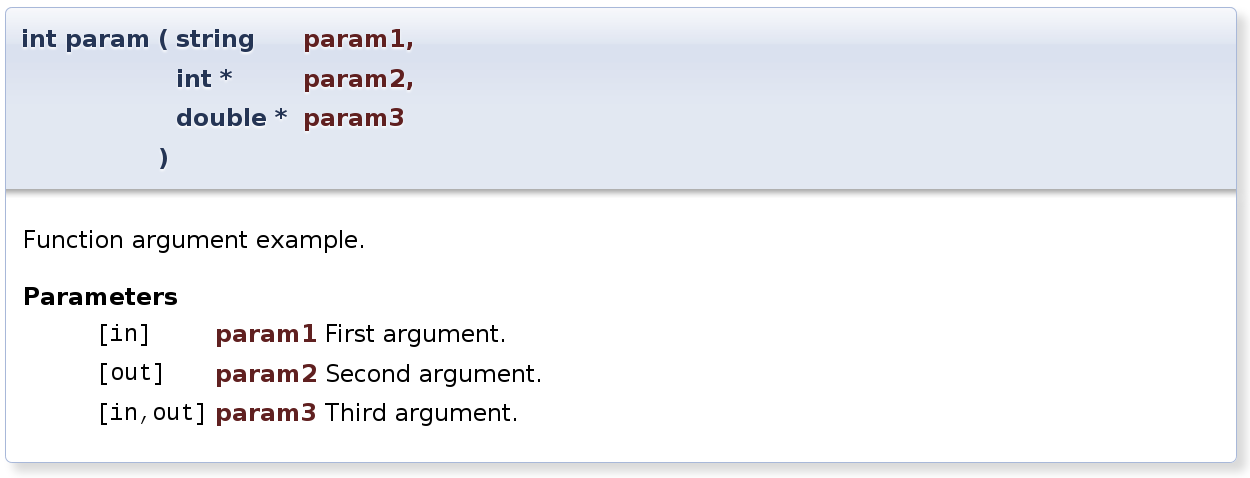
\includegraphics[width=0.8\textwidth]{write/document-the-code/function/param}
	\caption[پارامترهای یک تابع]{
		پارامترهای یک تابع.
	}
	\label{write/document-the-code/function/param}
\end{figure}

توصیف پارامتر ورودی از ساختار خاصی پیروی نمی‌کند و می‌تواند شامل تمام دستورهای
زیبا سازی متن باشد.
تمام برچسب‌های \lr{param} که پست سر هم قرار می‌گیرند با هم ادغام شده و به صورت یک 
بخش مستقل در مستند ظاهر می‌شوند.
در این بخش مستند توصیف هر پارامتر از یک خط جدید آغاز می‌شود.
شروع یک برچسب و یا بخش دیگر انتهای توصیف این برچسب را تعیین می‌کند.

در بسیاری از موارد چندین پارامتر برای نمایش یک موجودیت به کار گرفته می‌شوند.
برای نمونه یک نقطه در فضای سه بعدی با استفاده از سه عدد نمایش داده می‌شود.
در این حالت می‌توان نام چندین پارامتر را به صورت هم زمان به عنوان ورودی نام 
برای این برچسب به کار برد.
نام پارامترها در این حالت با استفاده از کاما از یکدیگر جدا می‌شود.
در زیر یک نمونه آورده شده است که در آن سه پارامتر با هم مستند شده است.
مستند تولید شده برای این نمونه نیز در شکل 
\ref{write/document-the-code/function/param-multi-with-single-tag} نمایش داده شده است.
\begin{C++}
/**
 * \brief Multiple parameter with single param tag.
 * \param x,y,z Coordinates of the position in 3D space.
 * \param t     Time of event.
 */
void param2(double x,double y,double z,double t);
\end{C++}

\begin{figure}
	\centering
	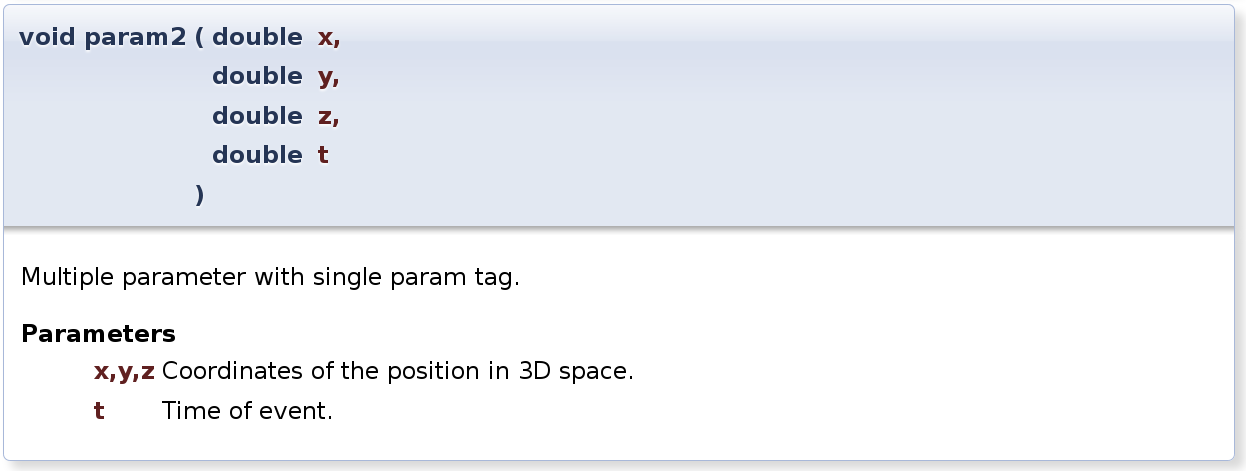
\includegraphics[width=0.8\textwidth]{write/document-the-code/function/param-multi-with-single-tag}
	\caption[پارامترهای یک تابع]{
		پارامترهای یک تابع. زمانی که چندین پارامتر برای یک کار مشترک به کار گرفته می‌شود
		می‌توان تمام آنها را به صورت یکجا مستند کرد. در این نمونه یک نقطه سه بعدی با سه 
		عدد صحیح نمایش داده شده است و در مستند فنی هر سه با هم مستند شده.
	}
	\label{write/document-the-code/function/param-multi-with-single-tag}
\end{figure}



\subsection{خروجی}
% return
% \return { description of the return value }

در اغلب زبان‌های برنامه سازی همه منظوره، یک نوع داده به عنوان نوع داده خروجی تابع
در نظر گرفته می‌شود.
در مستند سازی فنی برچسب \lr{return} برای مستند کردن خروجی تابع در نظر گرفته شده است.
ساختار کلی استفاده از این برچسب به صورت زیر است:
\begin{C++}
\return { description of the return value }
\end{C++}

ساختار متن توصیف خروجی یک تابع، از ساختار خاصی پیروی نمی‌کند و می‌تواند شامل
انواع برچسب‌های زیبا سازی متن باشد.
بر خلاف اینکه بسیاری از زبانهای مشهور مانند \lr{java}، \lr{C/C++} و \lr{C\#} تنها از 
یک نوع داده خروجی حمایت می‌کنند، امکان استفاده مکرر از این برچسب نیز وجود دارد.
در فرآیند تولید مستند فنی، تمام برچسب‌های \lr{return} که به صورت متوالی ظاهر شده‌اند
با یکدیگر ترکیب شده و در یک بخش نمایش داده می‌شوند.
متن توصیف خروجی تابع با شروع بخش جدید و یا یک برچسب دیگر، پایان می‌یابد.

در \lr{Doxygen} یک برچسب دیگر به نام \lr{returns} برای تشریح خروجی‌های یک تابع در نظر گرفته شده است.
از این برچسب زمانی استفاده می‌شود که بیش از یک خروجی برای یک تابع در نظر گرفته شده است.
ساختار کلی این برچسب به صورت زیر است:
\begin{C++}
\returns { description of the return value }
\end{C++}

\begin{note}
برچسب \lr{returns} کاملا شبیه به \lr{return} است و ویژگی خاصی ندارد. 
زمانی که تعداد خروجی‌های بیش از یکی باشد این برچسب مستند زیباتر و قابل درکی را 
ایجاد می‌کند.
\end{note}

\subsection{استثناها}
% throw
% exception
% \exception <exception-object> { exception description }

با ظهور زبان‌های برنامه سازی، راهکارهایی برای مدیریت خطا پیشنهاد شد که در آن
یک تابع خطا را تولید یک خروجی خاص نمایش می‌داد.
این نوع خروجی را \glspl{exception} می‌نامند که در زبان‌های برنامه سازی راهکاری متفاوت
از خروجی‌های معمولی را برای آنها در نظر می‌گیرند.
نکته‌ای که در مستند سازی فنی باید به آن توجه داشت این است که تمام استثناهای یک
تابع باید به صورت کامل مستند شود.
برای مستند کردن \glspl{exception} از برچسب \lr{exception} استفاده می‌شود.
ساختار کلی این برچسب به صورت زیر است:
\begin{C++}
\exception <exception-object> { exception description }
\end{C++}

دو پارامتر ورودی برای این برچسب در نظر گرفته شده که به ترتیب نام و توصیف استثنا
است.
وجود یک استثنا در یک تابع بررسی نمی‌شود از این رو مستند ساز باید در
مستند کردن استثنا دقت کند.
پاراگراف توصیف استثنا از ساختار خاصی پیروی نمی‌کند و می‌توان از برچسب‌های دیگر مانند
برچسب‌های زیبا سازی متن در آن استفاده کرد.
متن توصیف یک استثنا با رسیدن به یک خط خالی، بخش جدید و یا برچسب دیگر پایان می‌پذیرد.

معمولا توابع انواع متفاوتی استثنا تولید می‌کنند که هر یک حالت خاصی را نمایش می‌دهد.
از این رو امکان استفاده از چندین برچسب \lr{exception} فراهم شده است.
در فرآیند تولید مستند فنی، برچسب‌هایی که به صورت متوالی ظاهر شده‌اند با هم ترکیب
شده و در یک بخش نمایش داده می‌شوند.
در این حالت توصیف هر استثنا با شروع یک خط جدید آغاز می‌شود.
در نمونه زیر تابعی با دو نوع استثنا متفاوت مستند شده است و خروجی معادل با آن در شکل 
\ref{write/document-the-code/function/exception} نمایش داده شده است.
\begin{C++}
/**
 * \brief exception explanation
 *
 * \exception Exp1 Exception should be discussed here.
 * \exception Exp2 Exception should be discussed here.
 * \exception Exp3 Exception should be discussed here.
 *
 * This section causes new exception section to be generated by Doxygen.
 *
 * \exception Exp4 Exception should be discussed here.
 * \exception Exp5 Exception should be discussed here.
 */
int excetpion(Param p1, Param p2);
\end{C++} 
\begin{figure}
	\centering
	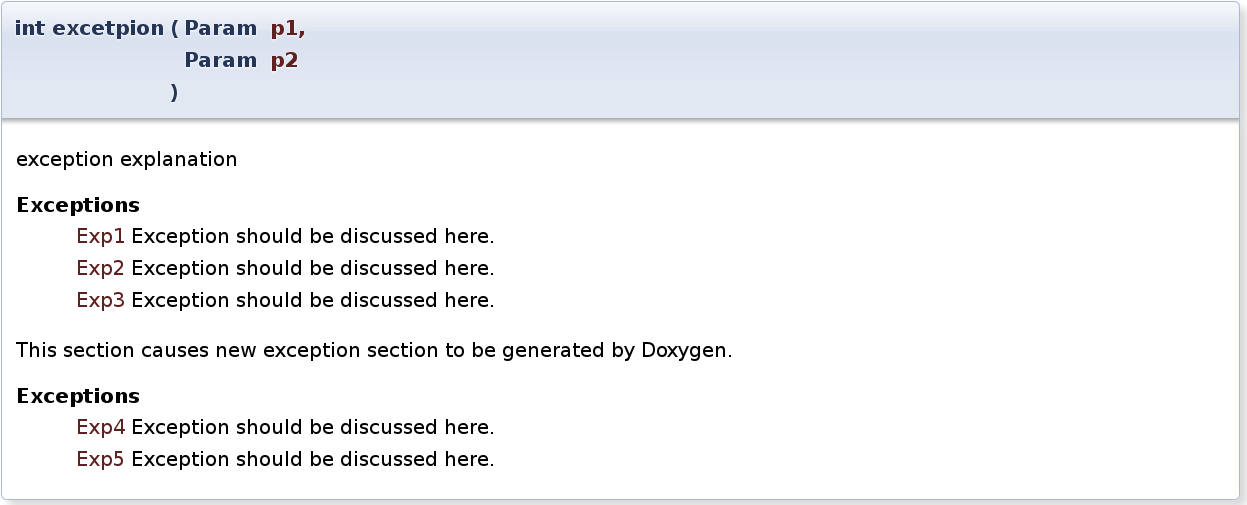
\includegraphics[width=0.8\textwidth]{write/document-the-code/function/exception}
	\caption[استثناهای یک تابع]{
		برچسب‌های \lr{exception} که به صورت پشت سر هم اورده شده است با یک دیگر ترکیب شده 
		و در یک بخش نمایش داده می‌شود.
	}
	\label{write/document-the-code/function/exception}
\end{figure}

برخی از ابزارهای مستند سازی از برچسب \lr{throw} برای توصیف یک استثنا استفاده می‌شود.
شاید دلیل این کار کلمه ذخیره شده \lr{throw} است که برای تولید یک استثنا در برخی
از زبان‌های برنامه سازی مانند \lr{C++} و \lr{java} استفاده می‌شود.
در \lr{Doxygen} نیز از این برچسب حمایت می‌شود.
ساختار کلی این برچسب به صورت زیر است:
\begin{C++}
\throw <exception-object> { exception description }
\end{C++}

زمانی که تعداد استثناها بیش از یکی باشد، می‌توان از برچسب \lr{throws} نیز استفاده کرد.

% TODO: maso 1392: پیش نیاز و پس نیاز یک تابع
% \subsection{پیش نیاز و پس نیاز}
% \post { description of the postcondition }
% 
% Starts a paragraph where the postcondition of an entity can be described. The
% paragraph will be indented. The text of the paragraph has no special internal
% structure. All visual enhancement commands may be used inside the paragraph.
% Multiple adjacent \post commands will be joined into a single paragraph. Each
% postcondition will start on a new line. Alternatively, one \post command may
% mention several postconditions. The \post command ends when a blank line or some
% other sectioning command is encountered.
% 
% \pre { description of the precondition }
% 
% Starts a paragraph where the precondition of an entity can be described. The
% paragraph will be indented. The text of the paragraph has no special internal
% structure. All visual enhancement commands may be used inside the paragraph.
% Multiple adjacent \pre commands will be joined into a single paragraph. Each
% precondition will start on a new line. Alternatively, one \pre command may
% mention several preconditions. The \pre command ends when a blank line or some
% other sectioning command is encountered.


% TODO: maso 1392: گراف فراخوانی یک تابع
% \subsection{گراف فراخوانی}
% callgraph
% callergraph
% \callgraph
% 
% When this command is put in a comment block of a function or method and HAVE_DOT
% is set to YES, then doxygen will generate a call graph for that function
% (provided the implementation of the function or method calls other documented
% functions). The call graph will be generated regardless of the value of
% CALL_GRAPH.
% 
% Note
%     The completeness (and correctness) of the call graph depends on the doxygen
%     code parser which is not perfect.
% 
% See Also
%     section \callergraph.
% 
% \callergraph
% 
% When this command is put in a comment block of a function or method and HAVE_DOT
% is set to YES, then doxygen will generate a caller graph for that function
% (provided the implementation of the function or method calls other documented
% functions). The caller graph will be generated regardless of the value of
% CALLER_GRAPH.
% 
% Note
%     The completeness (and correctness) of the caller graph depends on the
%     doxygen code parser which is not perfect.
% 
% See Also
%     section \callgraph.








